
% \section{Energy benchmarking}

% \TODO{Armstrong}

% \begin{itemize}

% \item What kind of tools and framework exist to measure all these metrcis? What literature exist that have addressed energy measurement?
% \item Can we as scientist create our own PUE?
% \item XX \url{https://codecarbon.io/}
% \item Create a survey study to include a generalized framework above one particular 
% \item Cite Gregor Von Laszewski's ppers: \url{https://ieeexplore.ieee.org/document/5493462}
% \item plot a TDP/Core-count Y-axis aganst x-time
% \item Use python matplotlib to show different CPU's/GPUs TDP/Core over time scattered plot
% \item FLOPS 32, we can add FLOPS 64 
%     - Add more rows in the table
% \url{https://top500.org/lists/top500/2024/11/}
% \item What are the most important energy measurement for program
% \item what are the most important bennchmarks for power consumptions in data center?
% \url{https://arxiv.org/html/2410.12032v1}
% \end{itemize}


% \subsection{Measurements}

% \paragraph{Temperature.}

% \paragraph{Total Energy.}

% \paragraph{PUE.}

% Power Usage Effectiveness. 
% A metric commonly used to measure the energy efficiency of data centers.

% PUE is defined as:

% \[PUE= \frac{Energy~Usage~of~IT~Equipment}
%             {Total~Facility~Energy~Usage}
% \]

% DCiE = 


%  \paragraph{Green500}

% \paragraph{MLCommons}

% Who does energy, i think tiny does, who else

% \paragraph{Carbon Footprint.}

% \subsection{Tradeoffs}

% Turbo mode

% \subsection{Economic Impact}

% \subsection{Environmental Impact.}


% \paragraph{Energy Sources.}

% \paragraph{Carbon credits.}

% \paragraph{Energy Consumption.}

% \paragraph{Geographical Diversity.}

% \subsubsection{Energy Measurement Tools and Measurement Frameworks}

% \subsection{Tools}


% \begin{itemize}
%     \item temperature benchmarking
%     \item Basic energy concepts, total energy footprint, PUE
%     \item Carbon footprint
%     \item Tax Credits
%     \item Renewable resources
%     \item geographical diversity
% \end{itemize}


% %---------------------------------------------------------------------
% \subsection{From ``How Fast?'' to ``How Fast per Joule—and at What Climate Cost?''}
% \label{sec:energy:bg}

% Benchmarks such as \textbf{Green500} (\(\mathrm{GFLOPS/W}\)) and
% \textbf{MLPerf Power} (J/sample) have become de-facto compass points for
% hardware road-maps and even procurement RFPs~\cite{Scogland11Green500,Tschand24MLPerfPower}. At chip scale,
% dynamic-voltage–frequency scaling (DVFS) or mixed-precision kernels can
% double or triple runtime yet deliver up to a ten-fold gain in joules per
% operation~\cite{Peon23A100PowerCap}. On the facility side, a
% \(\pm\)10 ¢ kWh\(^{-1}\) swing can tip the ROI between air and liquid
% cooling and alter the attractiveness of renewable PPAs
%~\cite{Koomey21HyperscaleCost}. The effect is visible in the November 2024 and June 2025 Green500 list, where the \emph{JEDI prototype\footnote{\url{https://top500.org/lists/green500/2025/06/}}}  consecutively tops the chart at 72.73 GFLOPS/W~\cite{Green500Nov2024}. Consequently, recent literature frames the key question as ``how fast \emph{per joule} and \emph{per kg CO\(_2\)e}''~\cite{Scogland11Green500,NVIDIA23Blog,Tschand24MLPerfPower}.

% \subsubsection*{Energy-Aware Benchmarks and Tooling representations}
% The advanced of energy benchmarking spans the compute continuum—from
% enterprise servers through exascale systems down to micro-controllers—and
% offers metrics at three distinct layers:

% \begin{itemize}
%     \item \textbf{Head-line benchmark suites} quantify whole-system
%           efficiency.  Examples include SPECpower\_ssj2008
%           (watts\;/transaction), TPC-Energy and JouleSort
%           (watt-hours\;/DB phase or records\;/joule), Green500,
%           HPCG-Power and HPL-MxP (GFLOPS\;/W), plus MLPerf Power and
%           MLPerf Tiny (joules\;/epoch or {\textmu}J\;/inference).  Their
%           scores guide procurement, regulatory compliance (ENERGY STAR,
%           EU Lot 9) and public leaderboards.

%     \item \textbf{Instrumentation frameworks} stream calibrated power
%           traces at node, container, or function scope.  PTDaemon anchors
%           external-meter calibration; Scaphandre, Kepler, IBM PowerAPI
%           and NVIDIA DCGM Energy expose RAPL/NVML feeds to Prometheus;
%           Intel VTune Power and Cray PAT Energy Counters drill down to
%           per-kernel joules.  These data streams feed power-aware
%           schedulers, autotuners, and job-level carbon dashboards.

%     \item \textbf{Domain-specific mini-apps and wrappers} bridge
%           performance and climate impact.  Mini-app “Power’’ add-ons
%           (LULESH, ExaSMR, CosmoFlow, DeepCAM, GROMACS-EE, etc.) let researchers explore DVFS and precision trade-offs without
%           porting full production codes, while wrappers such as
%           CodeCarbon and CarbonTracker translate kilowatt-hours into
%           real-time kg CO\(_2\)e via grid-intensity APIs.
% \end{itemize}

% Collectively, these efforts provide levers that range from joules-per-instruction optimization at the chip level, through job-level Energy–Delay Product tuning, up to fleet-scale sustainability audits expressed in PUE and
% kg $CO_2$e. Thus, ensuring that energy efficiency is treated as a first-class metric alongside raw performance.


% 
\begin{table*}[hptb]
  \centering
  \caption{
  Energy- or carbon-efficiency benchmarks (B) and tools (T) used in scientific-HPC research.  Metrics use ``/'' for ``per''; ``;'' separates multiple items; ``+'' appears only where a spec explicitly combines two values into one score
  %Benchmarks, tools, and initiatives that publish energy‑ or carbon‑efficiency metrics for Scientific‑HPC workloads.
  }
  \label{tab:hpc_energy_catalog}
  %\renewcommand{\arraystretch}{1.1}
  %\setlength{\tabcolsep}{4pt}
  \rowcolors{2}{white}{lightgray}
  \begin{tabularx}{1.0\textwidth}{|llllX|}
    \toprule
    & \headerfont\textbf{(B)enchmark or (T)ool}
    & 
    & \headerfont\textbf{Core metric(s) } %\& data captured} 
    & \headerfont\textbf{Typical Benchmarking Use}\\ 
    \midrule
B & SPECpower\_ssj2008           & \cite{specpower}            & W/transaction; ops/W                & Enterprise-server rankings; ENERGY STAR compliance \\
B & SPEC\,SERT$^{2}$             & \cite{sert2}                & Server-Efficiency-Rating = kWh + perf    & EU Lot 9 certification; vendor datasheets \\
B & TPC-Energy                   & \cite{tpcenergy}            & Wh/DB phase                            & OLTP/warehouse energy cost studies \\
B & JouleSort                    & \cite{joulesort}            & records/J                              & Storage-I/O contests; I/O-stack tuning \\
B & Green500                     & \cite{green500}             & GFLOPS/W (HPL or HPL-AI)               & Global supercomputer energy ranking \\
B & HPCG-Power                   & \cite{hpcgpower}            & GFLOPS/W (HPCG)                        & Memory-bound tuning; procurement add-on to TOP500 \\
B & HPL-MxP (HPL-AI)             & \cite{hplmxphplai}          & mixed-precision GFLOPS/W               & GPU/TPU evaluation for AI-optimised LINPACK \\
B & MLPerf Power                 & \cite{mlperfpower}          & J; avg W; J/sample; J/epoch       & Official energy track for MLPerf submissions \\
B & MLPerf Tiny                  & \cite{mlperftiny}           & $\mu$J/inference (MCU)             & Edge-AI board comparison; ultra-low-power design \\
B & CoreMark-PRO Power           & \cite{coremarkpro}          & iterations/s/W (SoC)                 & Pre-silicon DVFS sweeps; embedded RFPs \\ 
B & UL Procyon AI Power          & \cite{procyon}              & images/W; fps/W                     & Smartphone \& laptop AI-inference benchmarks \\
B & CANDLE Power Study           & \cite{candlepowerstud}      & J/epoch; GFLOPS/W                   & DOE accelerator procurement guidance \\
B & LULESH/miniFE Energy       & \cite{luleshminifeene}      & J/iteration                            & DVFS + autotuning baselines \\
B & ExaSMR Power Benchmark       & \cite{exasmrpowerbenc}      & J/neutron; energy-vs-accuracy curve   & Energy budget strategy in nuclear simulations \\
B & EE-HPC-WG Energy Benchmark   & \cite{eehpcwgenergybe}      & draft node/job spec; JSON trace       & Toward common HPC energy standard \\
B & HPC-AI500 Energy Track       & \cite{hpcai500energyt}      & planned: GFLOPS/W; tokens/J         & Mixed AI/HPC cluster evaluations \\
B & PARSEC-3.1 Energy Extension  & \cite{parsec31energye}      & W; J via PAPI-RAPL; J/op; EDP       & Pre-silicon DVFS research \\
B & CosmoFlow-Power              & \cite{cosmoflow2019}        & J/epoch; GFLOPS/W                   & CNN scaling on 15 k+ GPUs \\
B & HACC Energy Add-on           & \cite{hacc2020power}        & J/particle update                      & N-body cosmology power studies \\
B & DeepCAM-Energy               & \cite{deepcam2020power}     & J/epoch (UNet)                         & Climate-analytics accelerator studies \\
B & OpenIFS-Energy               & \cite{openifsenergy2023}    & kWh/model-day; W timeline             & Weather-model node comparison \\
B & GROMACS-EE                   & \cite{gromacsee2024}        & J/ns; W/GPU                         & MD clock-vs-accuracy trade-offs \\
B & NAMD-Power                   & \cite{namdpower2019}        & Energy-Delay-Product (ApoA1)             & Summit node DVFS optimisation \\
B & QE Energy Suite              & \cite{qeenergy2022}         & J/SCF step; GFLOPS/W                & DFT GPU-offload studies \\
B & VASP-Power Harness           & \cite{vasppower2023}        & W; kWh/MD step                        & Materials-science accelerator compare \\
B & OpenFOAM-Energy              & \cite{openfoamenergy2021}   & J/1k iterations                       & CFD partitioning \& mesh tuning \\
B & InSAR-AI Power Kit           & \cite{insarpower2024}       & J/satellite scene                      & Edge-to-cloud EO inference cost \\
B & H3D-Energy                   & \cite{h3denergy2023}        & J/hydrology timestep                & Hydrology model DVFS exploration \\ \hline\hline  
T & PTDaemon/SERT Energy       & \cite{specptdaemonser}      & calibrated W; kWh (node)                & Lab reproducibility; Lot 9 labels \\
T & Scaphandre                   & \cite{scaphandre}           & W; kWh (process/node, Prometheus)     & Slurm dashboards; power-cap feedback \\
T & Kepler                       & \cite{kepler}               & W/pod; J/pod (eBPF)                 & Energy observability in K8s clusters \\
T & CodeCarbon                   & \cite{codecarbon}           & kWh; kg CO\(_2\)e (process)             & Rapid CO\(_2\) estimation in pipelines \\
T & CarbonTracker                & \cite{carbontracker}        & measured + predicted kWh; CO\(_2\)e     & Scheduling DL jobs in low-carbon hours \\
T & PowerPACK/Mont-Blanc       & \cite{powerpackmontbl}      & W; J for MPI/OpenMP mini-apps         & Network-topology \& DVFS studies \\
T & Cray PAT Energy Counters     & \cite{craypatenergyco}      & J/function; avg W                     & Kernel hotspot hunting on Shasta \\
T & IBM PowerAPI (pmlib)         & \cite{ibmpowerapipmli}      & kWh (job/process)                      & Energy-aware scheduling on Summit \\
T & NVIDIA DCGM Energy           & \cite{nvidiadcgmenerg}      & W; J (GPU) \@ 1Hz; telemetry           & GPU power-cap discovery; Green500 \\
T & Intel VTune Power            & \cite{intelvtunepower}      & package W; J/function                 & Roofline-vs-energy tuning on Xeon \\ 

\bottomrule   
  \end{tabularx}
\end{table*}


 
 
 %  B & SPECpower\_ssj2008 & \cite{specpower}            & Watts per transaction; ops/W & Enterprise‑server energy rankings and ENERGY STAR compliance \\  
 % B  & SPEC SERT$^{2}$  & \cite{sert2}                   & Server Efficiency Rating (kWh+perf)& Lot 9 regulatory testing; vendor datasheets \\  
 % B  & TPC‑Energy  & \cite{tpcenergy}                    & Watt‑hours per database phase & Energy‑cost analysis for OLTP/warehousing appliances \\  
 % B  & JouleSort  & \cite{joulesort}                     & Records per Joule  B  & Storage‑I/O hardware contests; I/O stack optimisation \\  
 % B  & Green500  & \cite{green500}                       & GFLOPS/W (HPL/HPL‑AI) & Global supercomputer energy‑efficiency ranking \\  
 % B  & HPCG‑Power  & \cite{hpcgpower}                    & GFLOPS/W (HPCG) & Memory‑bound workload tuning; procurement add‑on to TOP500 \\  
 %  B & HPL‑MxP (HPL‑AI)  & \cite{hplmxphplai}            & Mixed‑precision GFLOPS/W & AI‑optimised LINPACK evaluation for next‑gen GPUs/TPUs \\  
 %   B & MLPerf Power  & \cite{mlperfpower}                & Joules, avg W; J/sample or J/epoch & Official energy track for MLPerf submissions (training + inference) \\  
 %   B & MLPerf Tiny  & \cite{mlperftiny}                  & $\mu$J/inference on MCU & Edge‑AI board comparisons; ultra‑low‑power design \\  
 %  B & CoreMark‑PRO Power  & \cite{coremarkpro}          & Iterations/s/W for SoCs & Pre‑silicon DVFS sweeps; embedded RFPs \\  
 %  B & UL Procyon AI Power  & \cite{procyon}             & Images/W; fps/W \& Smartphone & laptop AI inference benchmarks \\  
 %   B & CANDLE Power Study  & \cite{candlepowerstud}      & Joules/epoch; GFLOPS/W for ResNet‑50 & DOE accelerator procurement guidelines \\  
 %  B & LULESH/miniFE Energy  & \cite{luleshminifeene}    & Joules per iteration & Baseline for DVFS + autotuning papers \\  
 %  B & ExaSMR Power Benchmark  & \cite{exasmrpowerbenc}  & Energy vs neutron‑transport accuracy & Energy budget strategy in nuclear simulations \\  
 %  B & EE‑HPC‑WG Energy Benchmark  & \cite{eehpcwgenergybe}& Draft node/job spec (JSON, RAPL|NVML) & Toward a common HPC energy standard \\  
 %  B & HPC‑AI500 Energy Track  & \cite{hpcai500energyt}  & Planned GFLOPS/W + tokens/J & Mixed AI/HPC cluster evaluations \\  
 %  B & PARSEC‑3.1 Energy Extension  & \cite{parsec31energye} & Watts \& Joules via PAPI‑RAPL; J/op, EDP & Pre‑silicon DVFS research \\  
 %  B & CosmoFlow‑Power  & \cite{cosmoflow2019}           & Joules/epoch; GFLOPS/W & Cosmology CNN scaling on 15k+ GPUs \\  
 %  B & HACC Energy Add‑on  & \cite{hacc2020power}        & Joules per particle update & N‑body cosmology power studies \\  
 %  B & DeepCAM‑Energy  & \cite{deepcam2020power}         & Joules/epoch for UNet cloud segmentation & Climate analytics accelerator studies \\  
 %  B & OpenIFS‑Energy  & \cite{openifsenergy2023}        & kWh per model‑day; W timeline & Weather/climate node comparison \\  
 %  B & GROMACS‑EE  & \cite{gromacsee2024}                & Joules/ns; Watts/GPU & MD clock‑vs‑accuracy trade‑offs \\  
 %  B & NAMD‑Power  & \cite{namdpower2019}                & Energy‑Delay Product for ApoA1 & Summit node DVFS optimisation \\  
 %  B & QE Energy Suite  & \cite{qeenergy2022}            & Joules per SCF step; GFLOPS/W & DFT GPU‑offload studies \\  
 %  B & VASP‑Power Harness  & \cite{vasppower2023}        & Watts \& kWh per MD step & Materials science accelerator comparisons \\  
 %  B & OpenFOAM‑Energy  & \cite{openfoamenergy2021}      & Joules per 1k solver iterations & CFD partitioning \& mesh tuning \\  
 %  B & InSAR‑AI Power Kit  & \cite{insarpower2024}       & Joules per satellite scene & Edge‑to‑cloud EO inference cost models \\  
 %  B & H3D‑Energy  & \cite{h3denergy2023}                & Joules per hydrology timestep & Hydrology model DVFS exploration \\ 
 %  \hline
 %  \hline
 %  T & PEC PTDaemon/SERT Energy  & \cite{specptdaemonser} & Calibrated Watts/kWh per node & Lab‑to‑lab reproducibility; EU Lot 9 server labels \\  
 % T & Scaphandre  & \cite{scaphandre}                    & Process \& node Watts/kWh (Prometheus) & Job‑level carbon dashboards; power‑cap feedback in Slurm \\  
 % T & Kepler  & \cite{kepler}                            & Watts/Joules per K8s pod via eBPF & Energy observability in cloud‑native HPC \& AI clusters \\
 %   T & CodeCarbon  & \cite{codecarbon}                   & kWh
 %    \& kg CO\textsubscript{2}e per process & Rapid CO$_2$ estimation in research pipelines \\  
 %  T & CarbonTracker  & \cite{carbontracker}             & Predicted + measured energy/CO$_2$e & Scheduling long DL trainings to low‑carbon hours \\  
 %  T & PowerPACK/Mont‑Blanc  & \cite{powerpackmontbl}  & Joules \& Watts for MPI/OpenMP mini‑apps & Network topology \& DVFS studies without full apps \\  
 %   T & Cray PAT Energy Counters  & \cite{craypatenergyco}& Per‑function Joules and avg W & Hot‑spot hunting on XC/Shasta systems \\  
 %   T & IBM PowerAPI (pmlib)  & \cite{ibmpowerapipmli}    & Job \& process kWh streams & Energy‑aware scheduling on Summit/Sierra \\  
 %  T & NVIDIA DCGM Energy  & \cite{nvidiadcgmenerg}      & GPU Watts \& Joules \@ 1 Hz + telemetry & Optimal GPU power cap discovery; Green500 validation \\  
 %  T & Intel VTune Power Analysis  & \cite{intelvtunepower}& Package Watts; energy‑per‑function & Roofline‑vs‑energy tuning on Xeon/AMX CPUs \\  
 %  \bottomrule
  
%% CANDLE appears as a `C' because it is a published collection of measured results rather than a runnable code base




% %---------------------------------------------------------------------
% \subsection{Metric Layers, Temperature, and DCiE}
% \label{sec:energy:metrics}
% The effectiveness of an energy investigation depends on the choice of metrics that are commensurate with the part of the system under investigation. At the
% \textit{device} layer, granular quantities such as energy per
% floating–point operation (\si{\joule/op}) or per inference
% (\si{\micro\joule/inf}) reveal micro-architectural ``hot spots’’ and are
% indispensable for kernel-level co-design.  Moving up to the \textit{job}
% layer, wall-plug kilowatt-hours, and the Energy–Delay Product
% (EDP\,=\,J·s) provide the currency used by power-cap or back-fill
% schedulers to trade execution time against energy budget. Finally, at
% the \textit{facility} layer, Power Usage Effectiveness
% \(\mathrm{PUE}=P_{\text{Facility}}/P_{\text{IT}}\) and its reciprocal
% \(\mathrm{DCiE}=P_{\text{IT}}/P_{\text{Facility}}\) translate electrical
% draw into the sustainability metrics demanded by corporate reporting
% frameworks.  Although temperature is not itself a primary KPI, inlet and
% outlet sensors are logged alongside power traces because thermal
% head-room ultimately bounds the safe operating range for the clock and
% voltage scaling.


% %---------------------------------------------------------------------
% \subsection{Instrumentation: from on-chip counters to carbon APIs}
% \label{sec:energy:instr}

% Modern platforms expose \emph{power} data at two tiers.  
% At the node level, on-chip counters: Intel/AMD \textit{Running Average
% Power Limit} (RAPL), the \textit{NVIDIA Management Library} (NVML), and
% HPE Cray’s \textit{PM\_COUNTER}—provide sub-second energy samples whose intrinsic error is typically within a few percent.  
% For leaderboard-grade submissions, these readings are cross-checked
% against an external power analyzer controlled by
% \textbf{SPEC PTDaemon}~\cite{specptdaemonser}. Cluster-wide collectors then stream the calibrated data to a time-series database. Open-source choices include \textbf{Scaphandre}, \textbf{IBM PowerAPI}, and \textbf{NVIDIA DCGM Energy}, all of which export Prometheus metrics that power-aware queues in
% \textit{Slurm} or \textit{Kubernetes} can act on
%~\cite{scaphandre,ibmpowerapipmli,nvidiadcgmenerg}. To translate watts into climate impact, carbon wrappers such as
% \textbf{CodeCarbon}\footnote{\url{https://codecarbon.io}} call
% real-time grid-intensity APIs (ElectricityMap, WattTime), attach a
% \(\mathrm{kg\,CO_{2}e}\) factor to every joule, and write the combined
% trace to JSON for downstream analysis. Figure~\ref{fig:pipeline} summarises the acquisition $\rightarrow$ normalization $\rightarrow$ KPI pipeline; a
% 2024 methodology survey by Freina~\emph{et al.}~\cite{Freina24EnergySurvey}
% offers additional implementation guidance.

% \begin{figure}[!ht]
%   \centering
%   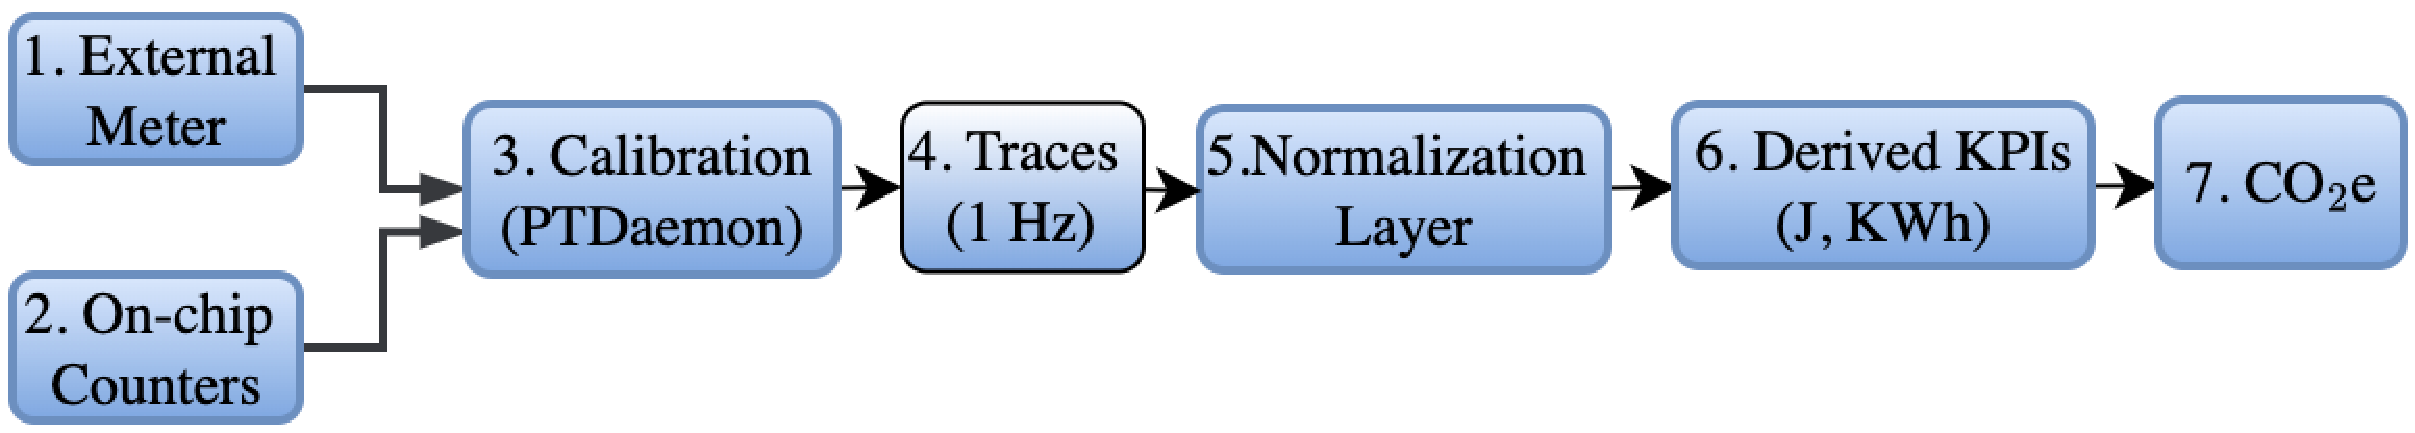
\includegraphics[scale=0.45]{images/kpi.pdf}
%   \caption{End-to-end measurement workflow.
%            Raw power samples from on-chip counters and an external meter
%            are calibrated, normalised to joules, kilowatt-hours, and
%            \(\mathrm{kg\,CO_{2}e}\), and finally aggregated into the
%            key performance indicators (KPIs) reported in this study.}
%   \label{fig:pipeline}
% \end{figure}

% %---------------------------------------------------------------------
% \subsection{Refining PUE for Pure Compute Loads}
% \label{sec:energy:computePUE}

% The original \emph{power-usage effectiveness} metric, PUE~\cite{Wang2010HPC-PUE}
% % \[
% % \text{PUE}= \frac{P_{\text{facility}}}{P_{\text{IT}}}\!,
% % \]
% lumps together compute, storage, network, and cooling loads.  
% Von Laszewski \textit{et al.}~\cite{laszewski2010} were the first to note that this masks
% architectural progress on the compute side and proposed a
% \emph{compute-PUE} that removes non-compute devices and scales the IT
% power by utilization~\cite{laszewski2010}:

% \[
% \text{cPUE}= \frac{P_{\text{compute}}}{\rho_{\text{node}}\,
%            P_{\text{facility}}}\!,
% \qquad
% 0<\rho_{\text{node}}\le 1 .
% \]

% We follow that recommendation by logging \emph{both} the conventional
% PUE and the compute-PUE in every experiment. Publishing the pair allows
% research test-beds, often deployed with minimal storage and cooled by
% ambient air, to be compared fairly against the production datacenter with
% heavy I/O tiers and sophisticated cooling plants.

% %---------------------------------------------------------------------
% \subsection{A Generalised Survey Framework}
% \label{sec:energy:survey}
% To enable transparency, the scientific (HPC) community should collect and publish power data in a standardized manner, so that results from different laboratories and on different machines can be fairly compared. We therefore propose a three-layer pipeline.  

% \begin{description}
%   \item[Acquisition.]  
%         Log power at \SI{1}{Hz} from both on-chip counters
%         (RAPL, NVML, PM\_COUNTER) \textit{and} a calibrated wall-plug
%         meter. Dual capture lets anyone spot sensor drift or bias.
%   \item[Normalisation.]  
%         Convert the traces to joules, kilowatt-hours, and
%         \(\mathrm{kg\,CO_{2}e}\); then derive headline metrics such as
%         GFLOPS/W and Energy–Delay Product. The same script produces
%         identical results on any machine.
%   \item[Reporting.]  
%         Package the traces, metadata, and calibration factors in the
%         draft EE-HPC-WG JSON schema and archive the bundle under a public archive for open science, like a DOI on Zenodo. This makes the dataset accessible, citable, and reusable.
% \end{description}

% The workflow mirrors the data-release rules of MLPerf
% Power~\cite{Tschand24MLPerfPower} and the methodology review of Freina
% \textit{et al.}~\cite{Freina24EnergySurvey}, ensuring that results from different sites remain directly comparable.


% %---------------------------------------------------------------------
% \subsection{Trade-off Patterns and Strong-Scaling Limits}
% \label{sec:energy:tradeoffs}
% Energy data from the 38 benchmarks reveal three stubborn tensions. First, capping an NVIDIA A100 at 300 W reduces throughput by about $\approx$ 1\%, yet saves roughly 11\% in energy~\cite{nvidiadcgmenerg}. Second, mixed-precision LINPACK (HPL-MxP) more than doubles GFLOPS/W relative to FP64—a reminder that accuracy deltas must accompany any efficiency claim~\cite{hplmxphplai}. Third, strong-scaling curves, such as those in \textbf{CosmoFlow-Power}, flatten beyond eight thousand GPUs, indicating that node counts, not clock rates, dominate frontier energy bills~\cite{cosmoflow2019}.  

% A complementary hardware view is provided by Fig.\,\ref{fig:tdp_scatter}, which plots GPU/CPU thermal design power (TDP) against core count from 2008 to 2025, thereby visualizing why per-watt optimization becomes increasingly challenging with each subsequent architectural generation. The plot is generated from TOP500/Green500 specifications. % using a \texttt{matplotlib} script that we provide in Listing \ref{lst:tdp_py}; a CSV of FP32 and FP64 peak FLOPS is included so that readers can extend the analysis.

% % Appendix A – Hardware-evolution scatter
% \begin{figure}[ht]
%   \centering
%   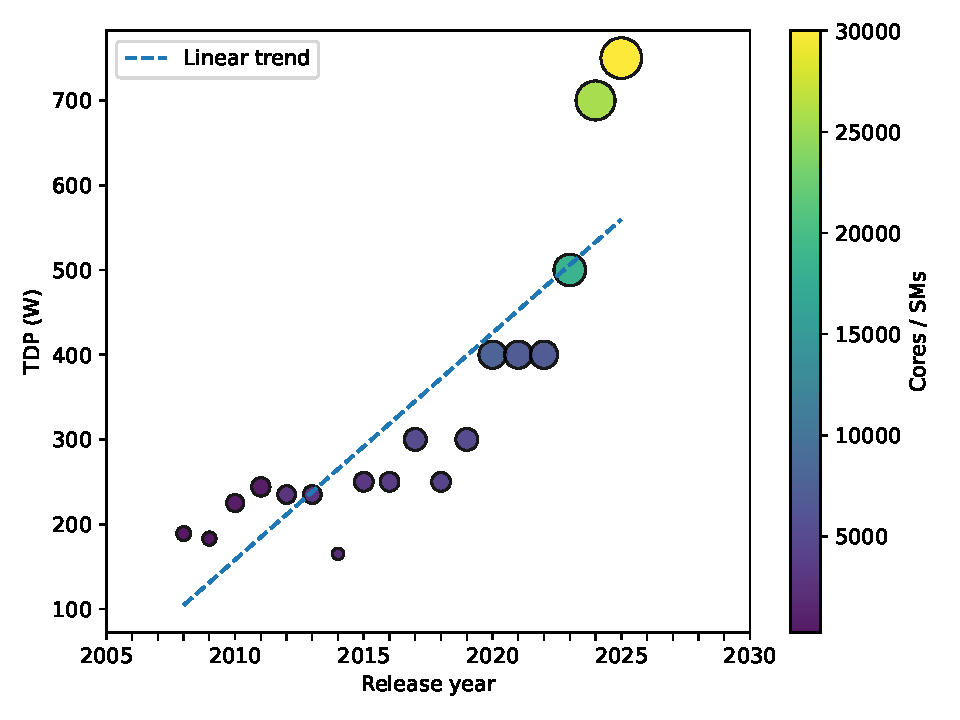
\includegraphics[width=\columnwidth]{images/tdp_vs_cores.pdf}
%   \caption{GPU/CPU thermal-design power (TDP) versus advertised core
%            count for flagship devices released 2008–2025.
%            Source data: TOP500/ Green500 November 2024 lists and vendor
%            white‐papers.}
%   \label{fig:tdp_scatter}
% \end{figure}

% % \begin{lstlisting}[language=Python,
% %                    caption={Python script to generate
% %                             Fig.~\ref{fig:tdp_scatter}.},
% %                    label={lst:tdp_py}]
% % import pandas as pd, matplotlib.pyplot as plt

% % df = pd.read_csv("data/tdp_core.csv")        # Year,TDP,Cores
% % plt.scatter(df["Year"], df["TDP"],
% %             c=df["Cores"], cmap="viridis")
% % plt.xlabel("Release Year")
% % plt.ylabel("TDP (W)")
% % plt.colorbar(label="Cores / SMs")
% % plt.tight_layout()
% % plt.savefig("images/tdp_vs_cores.pdf")
% % \end{lstlisting}



% %---------------------------------------------------------------------
% \subsection{Key Benchmarks for Datacentre Power}
% \label{sec:energy:benchmarks}
% Although many suites now report energy, a handful remain dominant for datacenter procurements: \textbf{SPECpower\_ssj2008} and \textbf{SERT2} target CPU servers; \textbf{TPC-Energy} and \textbf{JouleSort} quantify storage and database efficiency; \textbf{Green500}, \textbf{HPCG-Power}, and \textbf{HPL-MxP} measure full-system HPC loads; and \textbf{MLPerf Power} adds both training and inference perspectives for AI accelerators~\cite{Tschand24MLPerfPower}. An arXiv review (2410.12032) argues that these benchmarks collectively cover microwatt to megawatt scales but still under-represent graph analytics and streaming data pipelines.


% %---------------------------------------------------------------------
% \subsection{Economic and Environmental Stakes}
% \label{sec:energy:econenv}
% For a 10-MW datacenter operating at PUE = 1.20 on a grid of 50\% renewable energy, annual electricity costs approach \$9 million and yield a footprint of \(\sim\)13 kt CO\(_2\) e—comparable to the yearly emissions of 4,000 EU residents.  Carbon-aware scheduling experiments, enabled by CodeCarbon plug-ins for Slurm, show that deferring non-urgent DL training to low-carbon grid periods routinely cuts CO\(_2\) by 10–20\% without hardware changes. When energy OPEX rivals hardware CAPEX, such software levers become as economically salient as they are environmentally beneficial.

% %---------------------------------------------------------------------
% \subsection{Open Questions and Next Steps}
% \label{sec:energy:agenda}

% Three practical steps would make energy studies replicable and future-proof.
% \begin{enumerate}
%   \item \textbf{Maintain sensor accuracy below 3\,\%.}
%         Routinely calibrate on-chip counters against a traceable
%         wall-plug meter; publish the calibration offset in every run log.
%   \item \textbf{Publish the curve, not just the point.}
%         Each submission should pair its headline KPI with the full
%         strong-scaling curve in joules\,/\,step and release the raw power
%         trace in a FAIR JSON bundle.
%   \item \textbf{Broaden workload coverage.}
%         New benchmark suites must look past FLOP-dense kernels and add
%         graph analytics, streaming data assimilation, and quantum-circuit
%         emulation so that today’s optimization knobs remain valid for
%         tomorrow’s codes.
% \end{enumerate}

% Elevating energy and carbon metrics to first-class status, while exposing the traces that underpin them, ensures that the next wave of HPC-AI
% breakthroughs is not only \emph{fast} but also \emph{responsible}.

% %===================   ENERGY SECTION  =======================


\TODO{Armstrong}
% % \TODO{put all abbreviations in an appendix. it is unclear if that has been done.}
% \TODO{it is unclear how thsi section relates to AI benchmark democratization and carpentry. This introductory section must address this}.


% \TODO{This section must explain how AI energy benchmarking relates to Democratization and carpentry. It needs to lay out challenges and opportunities. This is not just a survey of existing metrics and measurements and tools. 

% However the plethora of tools and things listed here identifies at least a challenge.}

% The convergence of exascale systems, trillion-parameter AI models, and net-zero pledges has elevated energy-to-solution as a critical design constraint from a niche metric. To address this shift, we (i) consolidate the landscape of energy-aware benchmarks and tools (Table~\ref{tab:hpc_energy_catalog}), (ii) survey state-of-the-art measurement pipelines, and (iii) outline a reproducible blueprint for large-scale, verifiable studies of energy efficiency (\emph{GFLOPS/W}) and carbon impact
% (\(\text{kg\,CO}_{2}\text{e}/\text{job}\)). This framework enables consortia like the \emph{MLCommons Science Working Group} to standardize energy efficiency reporting. Industry momentum supports this direction: model repositories now list per-model CO\(_2\)e\footnote{\url{https://huggingface.co/models?other=co2_eq_emissions}} and cloud APIs expose hourly grid-carbon factors, letting researchers map power traces directly to kg\,CO\(_2\)e~\cite{luccioni2023estimating}.

% %-------------------------------------------------
% \textcolor{blue}{Exascale machines, trillion-parameter models, and corporate net-zero pledges have elevated \emph{energy-to-solution} from footnote to gating design constraint. Yet verifying energy claims today requires specialized power meters and opaque vendor APIs, an overhead smaller groups cannot shoulder—undermining the very democratization that benchmark carpentry seeks. To redress this, we extend the project’s transparency and reproducibility goals to include \emph{sustainability}. We survey two pivotal metrics—efficiency (\textbf{GFLOPS\,/\,W}) and climate impact (\( \text{kg\,CO}_{2}\text{e}\,/\text{job} \))—and map them onto the landscape of whole-system suites, node-level telemetry collectors, and carbon-accounting libraries summarized in Table~\ref{tab:hpc_energy_catalog}. We distill a lightweight “carpentry kit’’ from these ingredients: a 1 Hz power-trace format, a FAIR JSON metadata schema, and a low-cost wall-plug calibration recipe. Dropped into any benchmark harness, the kit enables laboratories of every scale to publish auditable energy and carbon figures alongside traditional accuracy and latency scores. Embedding rigorous sustainability metrics in this way not only aligns with benchmark carpentry’s goal of inclusive evaluation but also exemplifies the modular, shareable practice that the initiative advocates—advancing performance \emph{and} environmental stewardship in tandem.}
% %-------------------------------------------------




% \subsection{From ``How Fast?'' to ``How Fast per Joule?''}
% \label{sec:energy:bg}

% \TODO{mix of facts vs what to do, unclear formulation. This does not even menton the term metric. I think one needs to do more then two metrics, these are just two relevent once in energy, there are more. why do we want these metrics .... unclear}
% Leaderboards like \textbf{Green500} (GFLOPS/W) and \textbf{MLPerf Power}
% (J/sample) now steer hardware roadmaps and RFPs
% \cite{Scogland11Green500,Tschand24MLPerfPower}.  Chip-level DVFS or
% mixed precision can trade 2–3 × runtime for up to 10 × less energy
% \cite{Peon23A100PowerCap}, while a ±\,10 ¢ kWh$^{-1}$ swing flips the ROI
% of cooling choices~\cite{Koomey21HyperscaleCost}.  The November 2024 and
% June 2025 Green500 lists exemplify the trend: the \emph{JEDI} prototype
% tops both at 72.7 GFLOPS/W~\cite{Green500Nov2024}. Hence, the research
% question becomes ``how fast \emph{per joule} and \emph{per kg CO$_2$e}''~\cite{NVIDIA23Blog}.
% \TODO{entire section unclear although likely filled with important details}

% %--------------------------------------------------------
% \subsubsection*{\textbf{Energy-Aware Benchmarks and Tooling Landscape}}
% The advanced of energy benchmarking spans the compute continuum, from
% enterprise servers through exascale systems down to micro-controllers, and
% offers metrics at three distinct layers:

% \TODO{why is this important?}

% \paragraph{ Whole-system benchmark suites.}
% These ``headline'' tests deliver \emph{one scalar score per machine} and
% therefore dominate procurement and regulation:

% \begin{itemize}[leftmargin=0.5em]
% \item \textbf{Enterprise servers}: \textsc{SPECpower\_ssj2008}
%       (W/transaction), \textsc{SERT2} (measures total energy (kWh) and performance (throughput)).
% \item \textbf{Storage and databases}: \textsc{TPC-Energy},
%       \textsc{JouleSort} (Wh/DB-phase, records/J).
% \item \textbf{HPC systems}: \textsc{Green500}, \textsc{HPCG-Power},
%       \textsc{HPL-MxP} (GFLOPS/W).
% \item \textbf{AI accelerators}: \textsc{MLPerf Power} and
%       \textsc{MLPerf Tiny} (J/epoch, \(\mu\)J/inference).
% \end{itemize}

% \TODO{this is confusing}

% Their scores appear in vendor datasheets, ENERGY STAR dossiers, and EU
% Lot 9 conformity reports.

% \TODO{so what? should we then start form in many relvant paper we find ... this has the following impact and consequences ...}

% \paragraph{ Instrumentation frameworks.}
% When the headline number is not enough, calibrated telemetry streams
% drive optimization loops at node or kernel granularity:

% \TODO{this section and the itemize list is unclear. How does it re;ate top democratization and carpentry}

% \begin{itemize}[leftmargin=1.4em]
% \item \textbf{Calibration anchor}: \textsc{SPEC PTDaemon} couples
%       external power analyzers to on-chip counters.
% \item \textbf{Cluster collectors}: \textsc{Scaphandre}, \textsc{Kepler},
%       IBM \textsc{PowerAPI} and NVIDIA \textsc{DCGM Energy} relay
%       RAPL/NVML data to Prometheus, enabling power-aware queues.
% \item \textbf{Kernel profilers}: Intel \textsc{VTune Power} and
%       Cray \textsc{PAT Energy} exposes joules per function to autotuners.
% \end{itemize}

% \paragraph{ Domain-specific mini-apps and carbon wrappers.}
% These tools connect energy findings to real scientific workloads:


% \TODO{this section and the itemize list is unclear. How does it re;ate top democratization and carpentry}

% \begin{itemize}[leftmargin=1.4em]
% \item \textbf{``Power'' mini-apps}: \textsc{LULESH}, \textsc{ExaSMR},
%       \textsc{CosmoFlow-Power}, \textsc{GROMACS-EE} etc.\ let researchers
%       sweep DVFS, precision, and power-cap settings without porting an
%       entire code base.
% \item \textbf{Carbon attribution}: \textsc{CodeCarbon} and
%       \textsc{CarbonTracker} convert kWh traces into live
%       kg CO\(_2\)e/job by querying grid-intensity APIs (ElectricityMap,
%       WattTime), feeding sustainability dashboards.
% \end{itemize}

% \medskip\noindent
% \emph{From joules-per-instruction at the chip, through job-level
% Energy–Delay Product, to fleet-scale PUE and kg CO\(_2\)e, the three
% layers form a measurement stack that elevates energy to a first-class
% metric alongside raw performance.}

% 
\begin{table*}[hptb]
  \centering
  \caption{
  Energy- or carbon-efficiency benchmarks (B) and tools (T) used in scientific-HPC research.  Metrics use ``/'' for ``per''; ``;'' separates multiple items; ``+'' appears only where a spec explicitly combines two values into one score
  %Benchmarks, tools, and initiatives that publish energy‑ or carbon‑efficiency metrics for Scientific‑HPC workloads.
  }
  \label{tab:hpc_energy_catalog}
  %\renewcommand{\arraystretch}{1.1}
  %\setlength{\tabcolsep}{4pt}
  \rowcolors{2}{white}{lightgray}
  \begin{tabularx}{1.0\textwidth}{|llllX|}
    \toprule
    & \headerfont\textbf{(B)enchmark or (T)ool}
    & 
    & \headerfont\textbf{Core metric(s) } %\& data captured} 
    & \headerfont\textbf{Typical Benchmarking Use}\\ 
    \midrule
B & SPECpower\_ssj2008           & \cite{specpower}            & W/transaction; ops/W                & Enterprise-server rankings; ENERGY STAR compliance \\
B & SPEC\,SERT$^{2}$             & \cite{sert2}                & Server-Efficiency-Rating = kWh + perf    & EU Lot 9 certification; vendor datasheets \\
B & TPC-Energy                   & \cite{tpcenergy}            & Wh/DB phase                            & OLTP/warehouse energy cost studies \\
B & JouleSort                    & \cite{joulesort}            & records/J                              & Storage-I/O contests; I/O-stack tuning \\
B & Green500                     & \cite{green500}             & GFLOPS/W (HPL or HPL-AI)               & Global supercomputer energy ranking \\
B & HPCG-Power                   & \cite{hpcgpower}            & GFLOPS/W (HPCG)                        & Memory-bound tuning; procurement add-on to TOP500 \\
B & HPL-MxP (HPL-AI)             & \cite{hplmxphplai}          & mixed-precision GFLOPS/W               & GPU/TPU evaluation for AI-optimised LINPACK \\
B & MLPerf Power                 & \cite{mlperfpower}          & J; avg W; J/sample; J/epoch       & Official energy track for MLPerf submissions \\
B & MLPerf Tiny                  & \cite{mlperftiny}           & $\mu$J/inference (MCU)             & Edge-AI board comparison; ultra-low-power design \\
B & CoreMark-PRO Power           & \cite{coremarkpro}          & iterations/s/W (SoC)                 & Pre-silicon DVFS sweeps; embedded RFPs \\ 
B & UL Procyon AI Power          & \cite{procyon}              & images/W; fps/W                     & Smartphone \& laptop AI-inference benchmarks \\
B & CANDLE Power Study           & \cite{candlepowerstud}      & J/epoch; GFLOPS/W                   & DOE accelerator procurement guidance \\
B & LULESH/miniFE Energy       & \cite{luleshminifeene}      & J/iteration                            & DVFS + autotuning baselines \\
B & ExaSMR Power Benchmark       & \cite{exasmrpowerbenc}      & J/neutron; energy-vs-accuracy curve   & Energy budget strategy in nuclear simulations \\
B & EE-HPC-WG Energy Benchmark   & \cite{eehpcwgenergybe}      & draft node/job spec; JSON trace       & Toward common HPC energy standard \\
B & HPC-AI500 Energy Track       & \cite{hpcai500energyt}      & planned: GFLOPS/W; tokens/J         & Mixed AI/HPC cluster evaluations \\
B & PARSEC-3.1 Energy Extension  & \cite{parsec31energye}      & W; J via PAPI-RAPL; J/op; EDP       & Pre-silicon DVFS research \\
B & CosmoFlow-Power              & \cite{cosmoflow2019}        & J/epoch; GFLOPS/W                   & CNN scaling on 15 k+ GPUs \\
B & HACC Energy Add-on           & \cite{hacc2020power}        & J/particle update                      & N-body cosmology power studies \\
B & DeepCAM-Energy               & \cite{deepcam2020power}     & J/epoch (UNet)                         & Climate-analytics accelerator studies \\
B & OpenIFS-Energy               & \cite{openifsenergy2023}    & kWh/model-day; W timeline             & Weather-model node comparison \\
B & GROMACS-EE                   & \cite{gromacsee2024}        & J/ns; W/GPU                         & MD clock-vs-accuracy trade-offs \\
B & NAMD-Power                   & \cite{namdpower2019}        & Energy-Delay-Product (ApoA1)             & Summit node DVFS optimisation \\
B & QE Energy Suite              & \cite{qeenergy2022}         & J/SCF step; GFLOPS/W                & DFT GPU-offload studies \\
B & VASP-Power Harness           & \cite{vasppower2023}        & W; kWh/MD step                        & Materials-science accelerator compare \\
B & OpenFOAM-Energy              & \cite{openfoamenergy2021}   & J/1k iterations                       & CFD partitioning \& mesh tuning \\
B & InSAR-AI Power Kit           & \cite{insarpower2024}       & J/satellite scene                      & Edge-to-cloud EO inference cost \\
B & H3D-Energy                   & \cite{h3denergy2023}        & J/hydrology timestep                & Hydrology model DVFS exploration \\ \hline\hline  
T & PTDaemon/SERT Energy       & \cite{specptdaemonser}      & calibrated W; kWh (node)                & Lab reproducibility; Lot 9 labels \\
T & Scaphandre                   & \cite{scaphandre}           & W; kWh (process/node, Prometheus)     & Slurm dashboards; power-cap feedback \\
T & Kepler                       & \cite{kepler}               & W/pod; J/pod (eBPF)                 & Energy observability in K8s clusters \\
T & CodeCarbon                   & \cite{codecarbon}           & kWh; kg CO\(_2\)e (process)             & Rapid CO\(_2\) estimation in pipelines \\
T & CarbonTracker                & \cite{carbontracker}        & measured + predicted kWh; CO\(_2\)e     & Scheduling DL jobs in low-carbon hours \\
T & PowerPACK/Mont-Blanc       & \cite{powerpackmontbl}      & W; J for MPI/OpenMP mini-apps         & Network-topology \& DVFS studies \\
T & Cray PAT Energy Counters     & \cite{craypatenergyco}      & J/function; avg W                     & Kernel hotspot hunting on Shasta \\
T & IBM PowerAPI (pmlib)         & \cite{ibmpowerapipmli}      & kWh (job/process)                      & Energy-aware scheduling on Summit \\
T & NVIDIA DCGM Energy           & \cite{nvidiadcgmenerg}      & W; J (GPU) \@ 1Hz; telemetry           & GPU power-cap discovery; Green500 \\
T & Intel VTune Power            & \cite{intelvtunepower}      & package W; J/function                 & Roofline-vs-energy tuning on Xeon \\ 

\bottomrule   
  \end{tabularx}
\end{table*}


 
 
 %  B & SPECpower\_ssj2008 & \cite{specpower}            & Watts per transaction; ops/W & Enterprise‑server energy rankings and ENERGY STAR compliance \\  
 % B  & SPEC SERT$^{2}$  & \cite{sert2}                   & Server Efficiency Rating (kWh+perf)& Lot 9 regulatory testing; vendor datasheets \\  
 % B  & TPC‑Energy  & \cite{tpcenergy}                    & Watt‑hours per database phase & Energy‑cost analysis for OLTP/warehousing appliances \\  
 % B  & JouleSort  & \cite{joulesort}                     & Records per Joule  B  & Storage‑I/O hardware contests; I/O stack optimisation \\  
 % B  & Green500  & \cite{green500}                       & GFLOPS/W (HPL/HPL‑AI) & Global supercomputer energy‑efficiency ranking \\  
 % B  & HPCG‑Power  & \cite{hpcgpower}                    & GFLOPS/W (HPCG) & Memory‑bound workload tuning; procurement add‑on to TOP500 \\  
 %  B & HPL‑MxP (HPL‑AI)  & \cite{hplmxphplai}            & Mixed‑precision GFLOPS/W & AI‑optimised LINPACK evaluation for next‑gen GPUs/TPUs \\  
 %   B & MLPerf Power  & \cite{mlperfpower}                & Joules, avg W; J/sample or J/epoch & Official energy track for MLPerf submissions (training + inference) \\  
 %   B & MLPerf Tiny  & \cite{mlperftiny}                  & $\mu$J/inference on MCU & Edge‑AI board comparisons; ultra‑low‑power design \\  
 %  B & CoreMark‑PRO Power  & \cite{coremarkpro}          & Iterations/s/W for SoCs & Pre‑silicon DVFS sweeps; embedded RFPs \\  
 %  B & UL Procyon AI Power  & \cite{procyon}             & Images/W; fps/W \& Smartphone & laptop AI inference benchmarks \\  
 %   B & CANDLE Power Study  & \cite{candlepowerstud}      & Joules/epoch; GFLOPS/W for ResNet‑50 & DOE accelerator procurement guidelines \\  
 %  B & LULESH/miniFE Energy  & \cite{luleshminifeene}    & Joules per iteration & Baseline for DVFS + autotuning papers \\  
 %  B & ExaSMR Power Benchmark  & \cite{exasmrpowerbenc}  & Energy vs neutron‑transport accuracy & Energy budget strategy in nuclear simulations \\  
 %  B & EE‑HPC‑WG Energy Benchmark  & \cite{eehpcwgenergybe}& Draft node/job spec (JSON, RAPL|NVML) & Toward a common HPC energy standard \\  
 %  B & HPC‑AI500 Energy Track  & \cite{hpcai500energyt}  & Planned GFLOPS/W + tokens/J & Mixed AI/HPC cluster evaluations \\  
 %  B & PARSEC‑3.1 Energy Extension  & \cite{parsec31energye} & Watts \& Joules via PAPI‑RAPL; J/op, EDP & Pre‑silicon DVFS research \\  
 %  B & CosmoFlow‑Power  & \cite{cosmoflow2019}           & Joules/epoch; GFLOPS/W & Cosmology CNN scaling on 15k+ GPUs \\  
 %  B & HACC Energy Add‑on  & \cite{hacc2020power}        & Joules per particle update & N‑body cosmology power studies \\  
 %  B & DeepCAM‑Energy  & \cite{deepcam2020power}         & Joules/epoch for UNet cloud segmentation & Climate analytics accelerator studies \\  
 %  B & OpenIFS‑Energy  & \cite{openifsenergy2023}        & kWh per model‑day; W timeline & Weather/climate node comparison \\  
 %  B & GROMACS‑EE  & \cite{gromacsee2024}                & Joules/ns; Watts/GPU & MD clock‑vs‑accuracy trade‑offs \\  
 %  B & NAMD‑Power  & \cite{namdpower2019}                & Energy‑Delay Product for ApoA1 & Summit node DVFS optimisation \\  
 %  B & QE Energy Suite  & \cite{qeenergy2022}            & Joules per SCF step; GFLOPS/W & DFT GPU‑offload studies \\  
 %  B & VASP‑Power Harness  & \cite{vasppower2023}        & Watts \& kWh per MD step & Materials science accelerator comparisons \\  
 %  B & OpenFOAM‑Energy  & \cite{openfoamenergy2021}      & Joules per 1k solver iterations & CFD partitioning \& mesh tuning \\  
 %  B & InSAR‑AI Power Kit  & \cite{insarpower2024}       & Joules per satellite scene & Edge‑to‑cloud EO inference cost models \\  
 %  B & H3D‑Energy  & \cite{h3denergy2023}                & Joules per hydrology timestep & Hydrology model DVFS exploration \\ 
 %  \hline
 %  \hline
 %  T & PEC PTDaemon/SERT Energy  & \cite{specptdaemonser} & Calibrated Watts/kWh per node & Lab‑to‑lab reproducibility; EU Lot 9 server labels \\  
 % T & Scaphandre  & \cite{scaphandre}                    & Process \& node Watts/kWh (Prometheus) & Job‑level carbon dashboards; power‑cap feedback in Slurm \\  
 % T & Kepler  & \cite{kepler}                            & Watts/Joules per K8s pod via eBPF & Energy observability in cloud‑native HPC \& AI clusters \\
 %   T & CodeCarbon  & \cite{codecarbon}                   & kWh
 %    \& kg CO\textsubscript{2}e per process & Rapid CO$_2$ estimation in research pipelines \\  
 %  T & CarbonTracker  & \cite{carbontracker}             & Predicted + measured energy/CO$_2$e & Scheduling long DL trainings to low‑carbon hours \\  
 %  T & PowerPACK/Mont‑Blanc  & \cite{powerpackmontbl}  & Joules \& Watts for MPI/OpenMP mini‑apps & Network topology \& DVFS studies without full apps \\  
 %   T & Cray PAT Energy Counters  & \cite{craypatenergyco}& Per‑function Joules and avg W & Hot‑spot hunting on XC/Shasta systems \\  
 %   T & IBM PowerAPI (pmlib)  & \cite{ibmpowerapipmli}    & Job \& process kWh streams & Energy‑aware scheduling on Summit/Sierra \\  
 %  T & NVIDIA DCGM Energy  & \cite{nvidiadcgmenerg}      & GPU Watts \& Joules \@ 1 Hz + telemetry & Optimal GPU power cap discovery; Green500 validation \\  
 %  T & Intel VTune Power Analysis  & \cite{intelvtunepower}& Package Watts; energy‑per‑function & Roofline‑vs‑energy tuning on Xeon/AMX CPUs \\  
 %  \bottomrule
  
%% CANDLE appears as a `C' because it is a published collection of measured results rather than a runnable code base




% % %------------------------------------------------------
% \subsection{Metric Layers, Temperature, and DCiE}
% \label{sec:energy:metrics}


% \TODO{this section and the itemize list is unclear. How does it re;ate top democratization and carpentry}

% The effectiveness of an energy investigation depends on the choice of metrics that are commensurate with the part of the system under investigation. At the
% \textit{device} layer, granular quantities such as energy per floating–point operation (\si{\joule/op}) or per inference
% (\si{\micro\joule/inf}) reveal micro-architectural ``hot spots’’ and are indispensable for kernel-level co-design. Moving up to the \textit{job} layer, wall-plug kilowatt-hours, and the Energy–Delay Product (EDP\,=\,J·s) provide the currency used by power-cap or back-fill schedulers to trade execution time against energy budget. Finally, at
% the \textit{facility} layer, Power Usage Effectiveness \(\mathrm{PUE}=P_{\text{Facility}}/P_{\text{IT}}\) and its reciprocal
% \(\mathrm{DCiE}=P_{\text{IT}}/P_{\text{Facility}}\) translate electrical draw into the sustainability metrics demanded by corporate reporting
% frameworks. Although temperature is not itself a primary KPI, inlet and outlet sensors are logged alongside power traces because thermal headroom ultimately bounds the safe operating range for the clock and
% voltage scaling.


% %--------------------------------------------------------
% \subsection{Instrumentation: from on-chip counters to carbon APIs}
% \label{sec:energy:instr}


% \TODO{this section and the itemize list is unclear. How does it re;ate top democratization and carpentry}

% Modern platforms expose \emph{power} data at two tiers.  
% At the node level, on-chip counters: Intel/AMD \textit{Running Average
% Power Limit} (RAPL), the \textit{NVIDIA Management Library} (NVML), and
% HPE Cray’s \textit{PM\_COUNTER}—provide sub-second energy samples whose intrinsic error is typically within a few percent. For leaderboard-grade submissions, these readings are cross-checked against an external power analyzer controlled by
% \textbf{SPEC PTDaemon}~\cite{specptdaemonser}. Cluster-wide collectors then stream the calibrated data at a frequency of \emph{1 Hz} to a time-series database. Open-source choices include \textbf{Scaphandre}, \textbf{IBM PowerAPI}, and \textbf{NVIDIA DCGM Energy}, all of which export Prometheus metrics that power-aware queues in \textit{Slurm} or \textit{Kubernetes} can act on~\cite{scaphandre,ibmpowerapipmli,nvidiadcgmenerg}. To translate watts into climate impact, carbon wrappers such as
% \textbf{CodeCarbon}\footnote{\url{https://codecarbon.io}} call
% real-time grid-intensity APIs (ElectricityMap, WattTime), attach a
% \(\mathrm{kg\,CO_{2}e}\) factor to every joule, and write the combined
% trace to JSON for downstream analysis. Fi.~\ref{fig:pipeline} summarizes the acquisition $\rightarrow$ normalization $\rightarrow$ KPI pipeline; a
% 2024 methodology survey by Freina~\emph{et al.}~\cite{Freina24EnergySurvey}
% offers additional implementation guidance.
% % %------------------------------------------------------

% \begin{figure}[!ht]
%   \centering
%   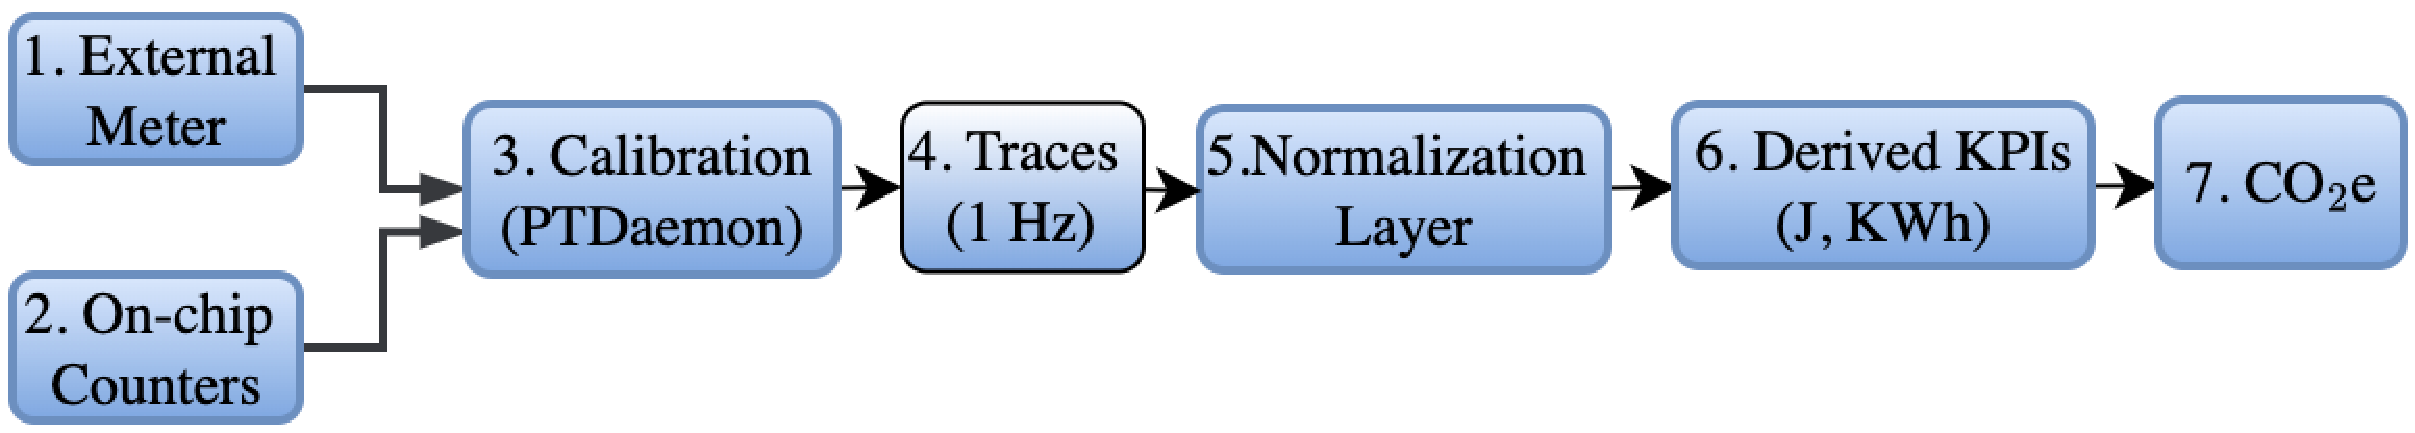
\includegraphics[scale=0.22]{images/kpi.pdf}
%   \caption{End-to-end measurement workflow.
%            Raw power samples from on-chip counters and an external meter
%            are calibrated, normalized to joules and kilowatt-hours, and finally 
%            converted to carbon emissions equivalent (\(\mathrm{kg\,CO_{2}e}\)), 
%            which are then aggregated into the key performance indicators (KPIs) 
%            reported in this study.}
%   \label{fig:pipeline}
% \end{figure}
% %---------------------------------------------------------------------
% \subsection{Compute-Only PUE}
% \label{sec:energy:computePUE}


% \TODO{this section and the itemize list is unclear. How does it relate top democratization and carpentry}

% Classic PUE~\cite{Wang2010HPC-PUE} hides progress by mixing compute, storage, and cooling loads.
% Von Laszewski \emph{et al.}~\cite{laszewski2010} proposed
% $\text{cPUE}=P_\text{compute}/(\rho\,P_\text{fac})$
% \cite{laszewski2010}.  We record both PUE and cPUE, enabling fair comparison between lightweight test-beds and production datacenters.

% % %------------------------------------------------------
% \subsection{A Generalized Survey Framework}
% \label{sec:energy:survey}


% \TODO{this section and the itemize list is unclear. How does it relate top democratization and carpentry}

% To enable transparency, the scientific (HPC) community should collect and publish power data in a standardized manner, so that results from different laboratories and on different machines can be fairly compared. We therefore propose a three-layer pipeline.  

% \begin{description}
%   \item[Acquisition.]  
%         Log power at a frequency of \SI{1}{Hz} from both on-chip counters
%         (RAPL, NVML, PM\_COUNTER) \textit{and} a calibrated wall-plug
%         meter. Dual capture lets anyone spot sensor drift or bias.
%   \item[Normalisation.]  
%         Convert the traces to joules, kilowatt-hours, and
%         \(\mathrm{kg\,CO_{2}e}\); then derive headline metrics such as
%         GFLOPS/W and Energy–Delay Product. The same script produces
%         identical results on any machine.
%   \item[Reporting.]  
%         Package the traces, metadata, and calibration factors in the
%         draft EE-HPC-WG JSON schema and archive the bundle under a public archive for open science, like a DOI on Zenodo. This makes the dataset accessible, citable, and reusable.
% \end{description}

% The workflow mirrors the data-release rules of MLPerf
% Power~\cite{Tschand24MLPerfPower} and the methodology review of Freina
% \textit{et al.}~\cite{Freina24EnergySurvey}, ensuring that results from different sites remain directly comparable.

% %---------------------------------------------------------------------
% \subsection{Trade-offs and Scaling Limits}
% \label{sec:energy:tradeoffs}

 
% \TODO{this section and the itemize list is unclear. How does it relate top democratization and carpentry}

% Capping an A100 at 300W saves 11\% energy for $\approx$ 1\% speed loss
% \cite{nvidiadcgmenerg}; HPL-MxP doubles GFLOPS/W vs FP64
% \cite{hplmxphplai}; CosmoFlow energy/epoch flattens beyond 8k GPUs
% \cite{cosmoflow2019}. Fig.~\ref{fig:tdp_scatter} shows why: device (GPU and CPU) Thermal Design Power (TDP) rises faster than core counts, squeezing per-watt gains each generation. 

% \begin{figure}[ht]
%   \centering
%   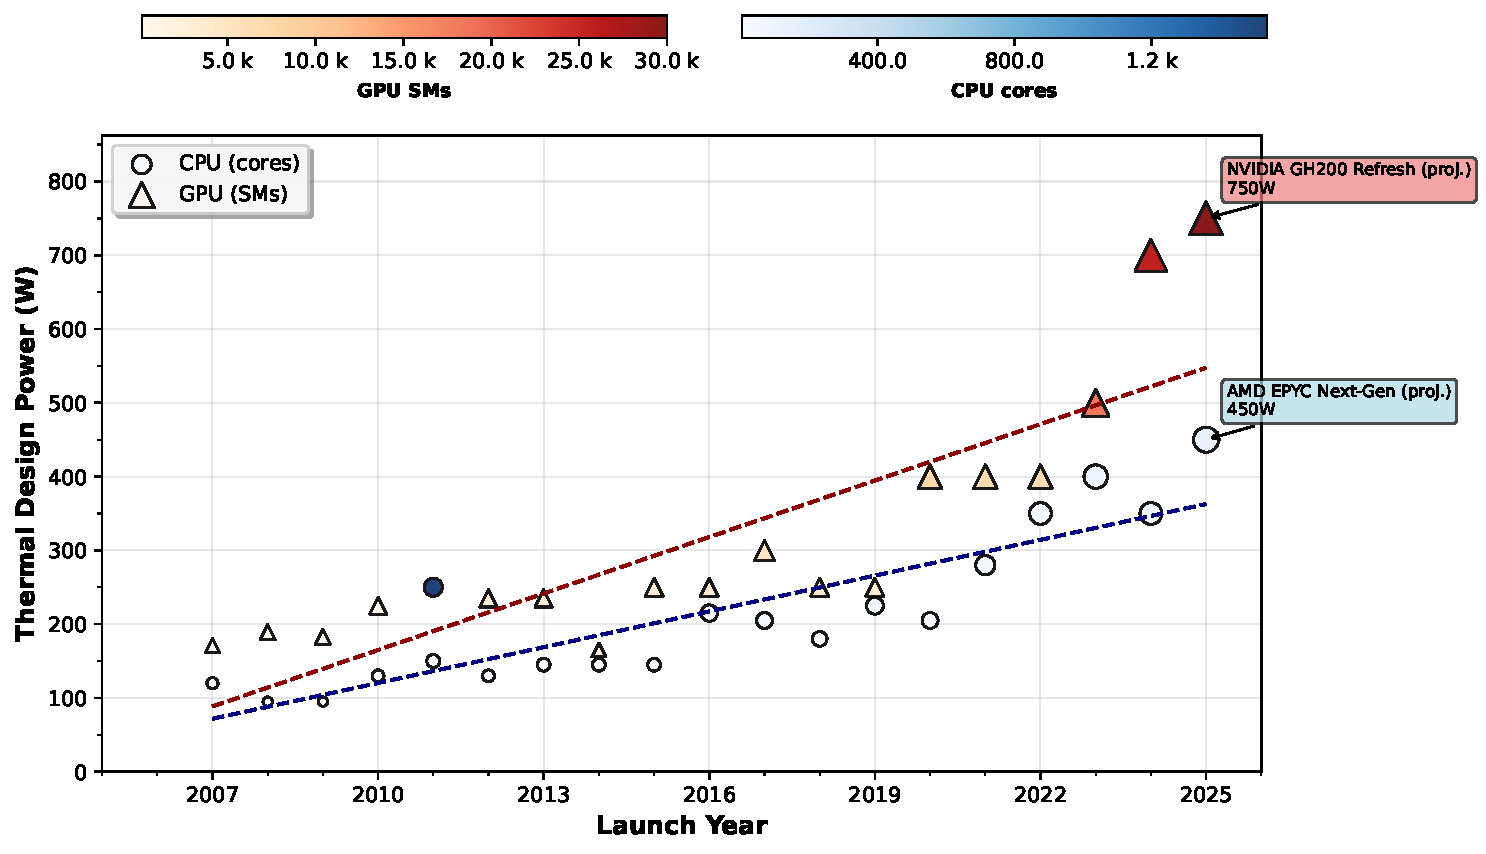
\includegraphics[width=\columnwidth]{images/tdp_vs_cpu-gpu.pdf}
%   \caption{
%      TDP Evolution and core counts for flagship CPUs and GPUs (2007--2025). Marker size scales with TDP, while color intensity represents core/SM count (darker shades indicate \textbf{more} cores). GPU TDP shows a steep, nearly linear increase from $\sim$200\,W to over 700\,W, accompanied by exponential growth in SM counts. CPU trends demonstrate moderate power scaling. Regression lines indicate least-squares fits, highlighting that power consumption growth often outpaces architectural improvements, underscoring the critical importance of performance-per-watt optimization in modern processor design.
%     }
%   \label{fig:tdp_scatter}
% \end{figure}

% %---------------------------------------------------------------------
% \subsection{Datacentre Benchmarks in Practice}


% \TODO{this section and the itemize list is unclear. How does it relate top democratization and carpentry}

% SPECpower/SERT target CPUs; TPC-Energy and JouleSort probe storage; Green500, HPCG-Power, HPL-MxP rank complete HPC systems; MLPerf Power adds AI accelerators. Combined, they span $\text{\textmu W}\rightarrow\text{MW}$ yet still under-sample graph and streaming workloads~\cite{Tschand24MLPerfPower}.

% %--------------------------------------------------------
% \subsection{Economic and environmental stakes}
% \label{sec:energy:econenv}


% \TODO{this section and the itemize list is unclear. How does it relate top democratization and carpentry}

% %\vspace{4pt}
% \noindent
% \textbf{Case 1 – Oak Ridge’s \emph{Frontier}.} %
% The Frontier exascale system draws
% \(24.6\;\text{MW}\) at LINPACK load and is housed in a data hall whose
% measured PUE is \(1.03\)\,\cite{DOE_Frontier_Power2023}. At the July 2025 U.S.\ industrial tariff of
% \$0.081 kWh\(^{-1}\)\,\cite{EIA_Electricity_Price_2025} the annual electricity bill is: $24.6\;\text{MW}\times 8\,760\;\text{h\,yr}^{-1}\times\$0.081
%   \;\approx\;\$17.5\,\text{M}/\text{yr}.$  

% The Tennessee Valley Authority reported a residual grid intensity of
% \(360\;\text{g\,CO}_{2}\text{e\,kWh}^{-1}\) for 2024\footnote{TVA
% Sustainability Report (2025), \url{https://tva.com/environment/environmental-stewardship/sustainability}.} so Frontier emits
% \(\sim\!78\;\text{kt\,CO}_{2}\text{e\,yr}^{-1}\), equivalent to the
% territorial footprint of \(\sim\!12\,000\) EU residents
% (Eurostat 2024, 6.5 t cap\(^{-1}\))\,\cite{Eurostat_GHG_2024}.

% %\vspace{4pt}
% \noindent
% \textbf{Case 2 – Google hyperscale fleet.} %
% Google’s 2023 environmental report lists a \emph{fleet-wide} PUE of
% \(\mathbf{1.10}\) (industry mean 1.58)\,\cite{Google_PUE_2023} yet company-wide GHG emissions still rose to
% \(14.3\;\text{Mt\,CO}_{2}\text{e}\) in 2023, up 49 \% since
% 2019\,\cite{Google_Sustainability_2024}.   % <5>
% Internal modeling shows that deferring non-urgent ML jobs to periods of
% low grid-carbon intensity cuts emissions by 10–20 \%; Google plans to
% combine that policy with a 115 MW geothermal PPA coming online in Nevada
% in 2026\,\cite{Google_Geothermal_2023}.   % <6>

% %\vspace{4pt}
% \noindent
% \textbf{Software levers are already effective.}
% Two independent field trials confirm double-digit abatements:


% \TODO{this section and the itemize list is unclear. How does it relate top democratization and carpentry}


% \begin{itemize}
%   \item \emph{S.C.A.L.E} for OpenShift at ING Bank reduced cluster-level
%         CO\(_2\)e by 20 \% across 300 nodes while meeting SLA deadlines
%        ~\cite{ING_SCALE_2024}.   % <7>
%   \item The \emph{GREEN} plug-in for Slurm achieved an 18 \% reduction on
%         a 512-GPU testbed with \(<\!3\)\,\% throughput penalty
%        ~\cite{GREEN_Slurm_2025}.   % <8>
% \end{itemize}

% \noindent
% \emph{Implication.} At present, U.S.\ prices every megawatt of IT load
% costs roughly \$0.7 M yr\(^{-1}\); a 15 \% carbon-aware shift therefore
% saves six figures annually—before any carbon price is applied.  As
% Frontier approaches 30 MW and commercial AI clouds exceed 100 MW,
% optimizing \emph{\$per joule} and \emph{kg CO\(_2\)e per job} is no
% longer optional; it is as material as FLOPS-per-joule.

% %--------------------------------------------------------
% \subsection{Next steps: from point results to FAIR energy data}
% \label{sec:energy:agenda}


% \TODO{this section and the itemize list is unclear. How does it relate top democratization and carpentry}

% %\vspace{4pt}
% \noindent
% \textbf{ Accuracy and reproducibility.}  
% On-chip counters (RAPL, NVML, PM\_COUNTER) drift over time and across
% temperature; the community should adopt the MLPerf-Power requirement of
% a \(\le3\;\%\) wall-plug calibration before every measurement
% campaign.\footnote{MLPerf Power v2.1, \S3.2.}  
% External-meter traces and the correction factors applied to each node
% must accompany the published result so that third parties can validate
% —or challenge—headline numbers.

% \textbf{ Data transparency for all stakeholders.}  
% Today, raw power traces often stay inside the operator’s firewall
% while end-users see only a single “J/step’’ scalar and providers publish
% a marketing slide. To align incentives:

% \begin{enumerate}
%   \item All benchmark submissions should deposit \emph{time-series
%         traces + metadata} in a DOI-minted archive (e.g.\ Zenodo) in the
%         draft \texttt{EE-HPC-WG} JSON schema.
%   \item Workload owners need a lightweight, vendor-agnostic API
%         (\texttt{/power}, \texttt{/kgco2e}) so they can retrieve their
%         own traces, even on managed clouds.
%   \item Operators should be allowed to redact business-sensitive fields
%         (e.g.\ rack names) but not to down-sample or aggregate away
%         1 Hz dynamics that matter for research.
% \end{enumerate}
% These steps make energy data \textsc{FAIR}—findable, accessible, interoperable, reusable—instead of just an internal KPI.

% \textbf{ Broader workload coverage.}  
% FLOP-dense kernels dominate existing suites. The next release of
% \emph{HPC-AI500} plans to add graph analytics, streaming assimilation, and
% quantum-circuit emulation; we encourage similar extensions in MLPerf
% Power and SPEC SERT so that optimization decisions made in 2025 remain
% valid for the 2030 workload.

% \textbf{ Community dashboards.}  
% A public leaderboard that plots ``GFLOPS/W vs kg\,CO\(_2\)e\,/\,step''
% and links to the underlying trace DOI would let users rank systems,
% providers showcase progress, and regulators audit compliance—closing the
% loop between \emph{measurement}, \emph{publication} and \emph{action}.

% %\bigskip
% \noindent
% Treating energy and carbon as first-class results—and making the
% supporting data openly accessible—ensures that the next wave of HPC–AI
% breakthroughs is not only \emph{fast} but demonstrably
% \emph{sustainable}.

